\begin{figure*}[!t]
\small
  \centering
  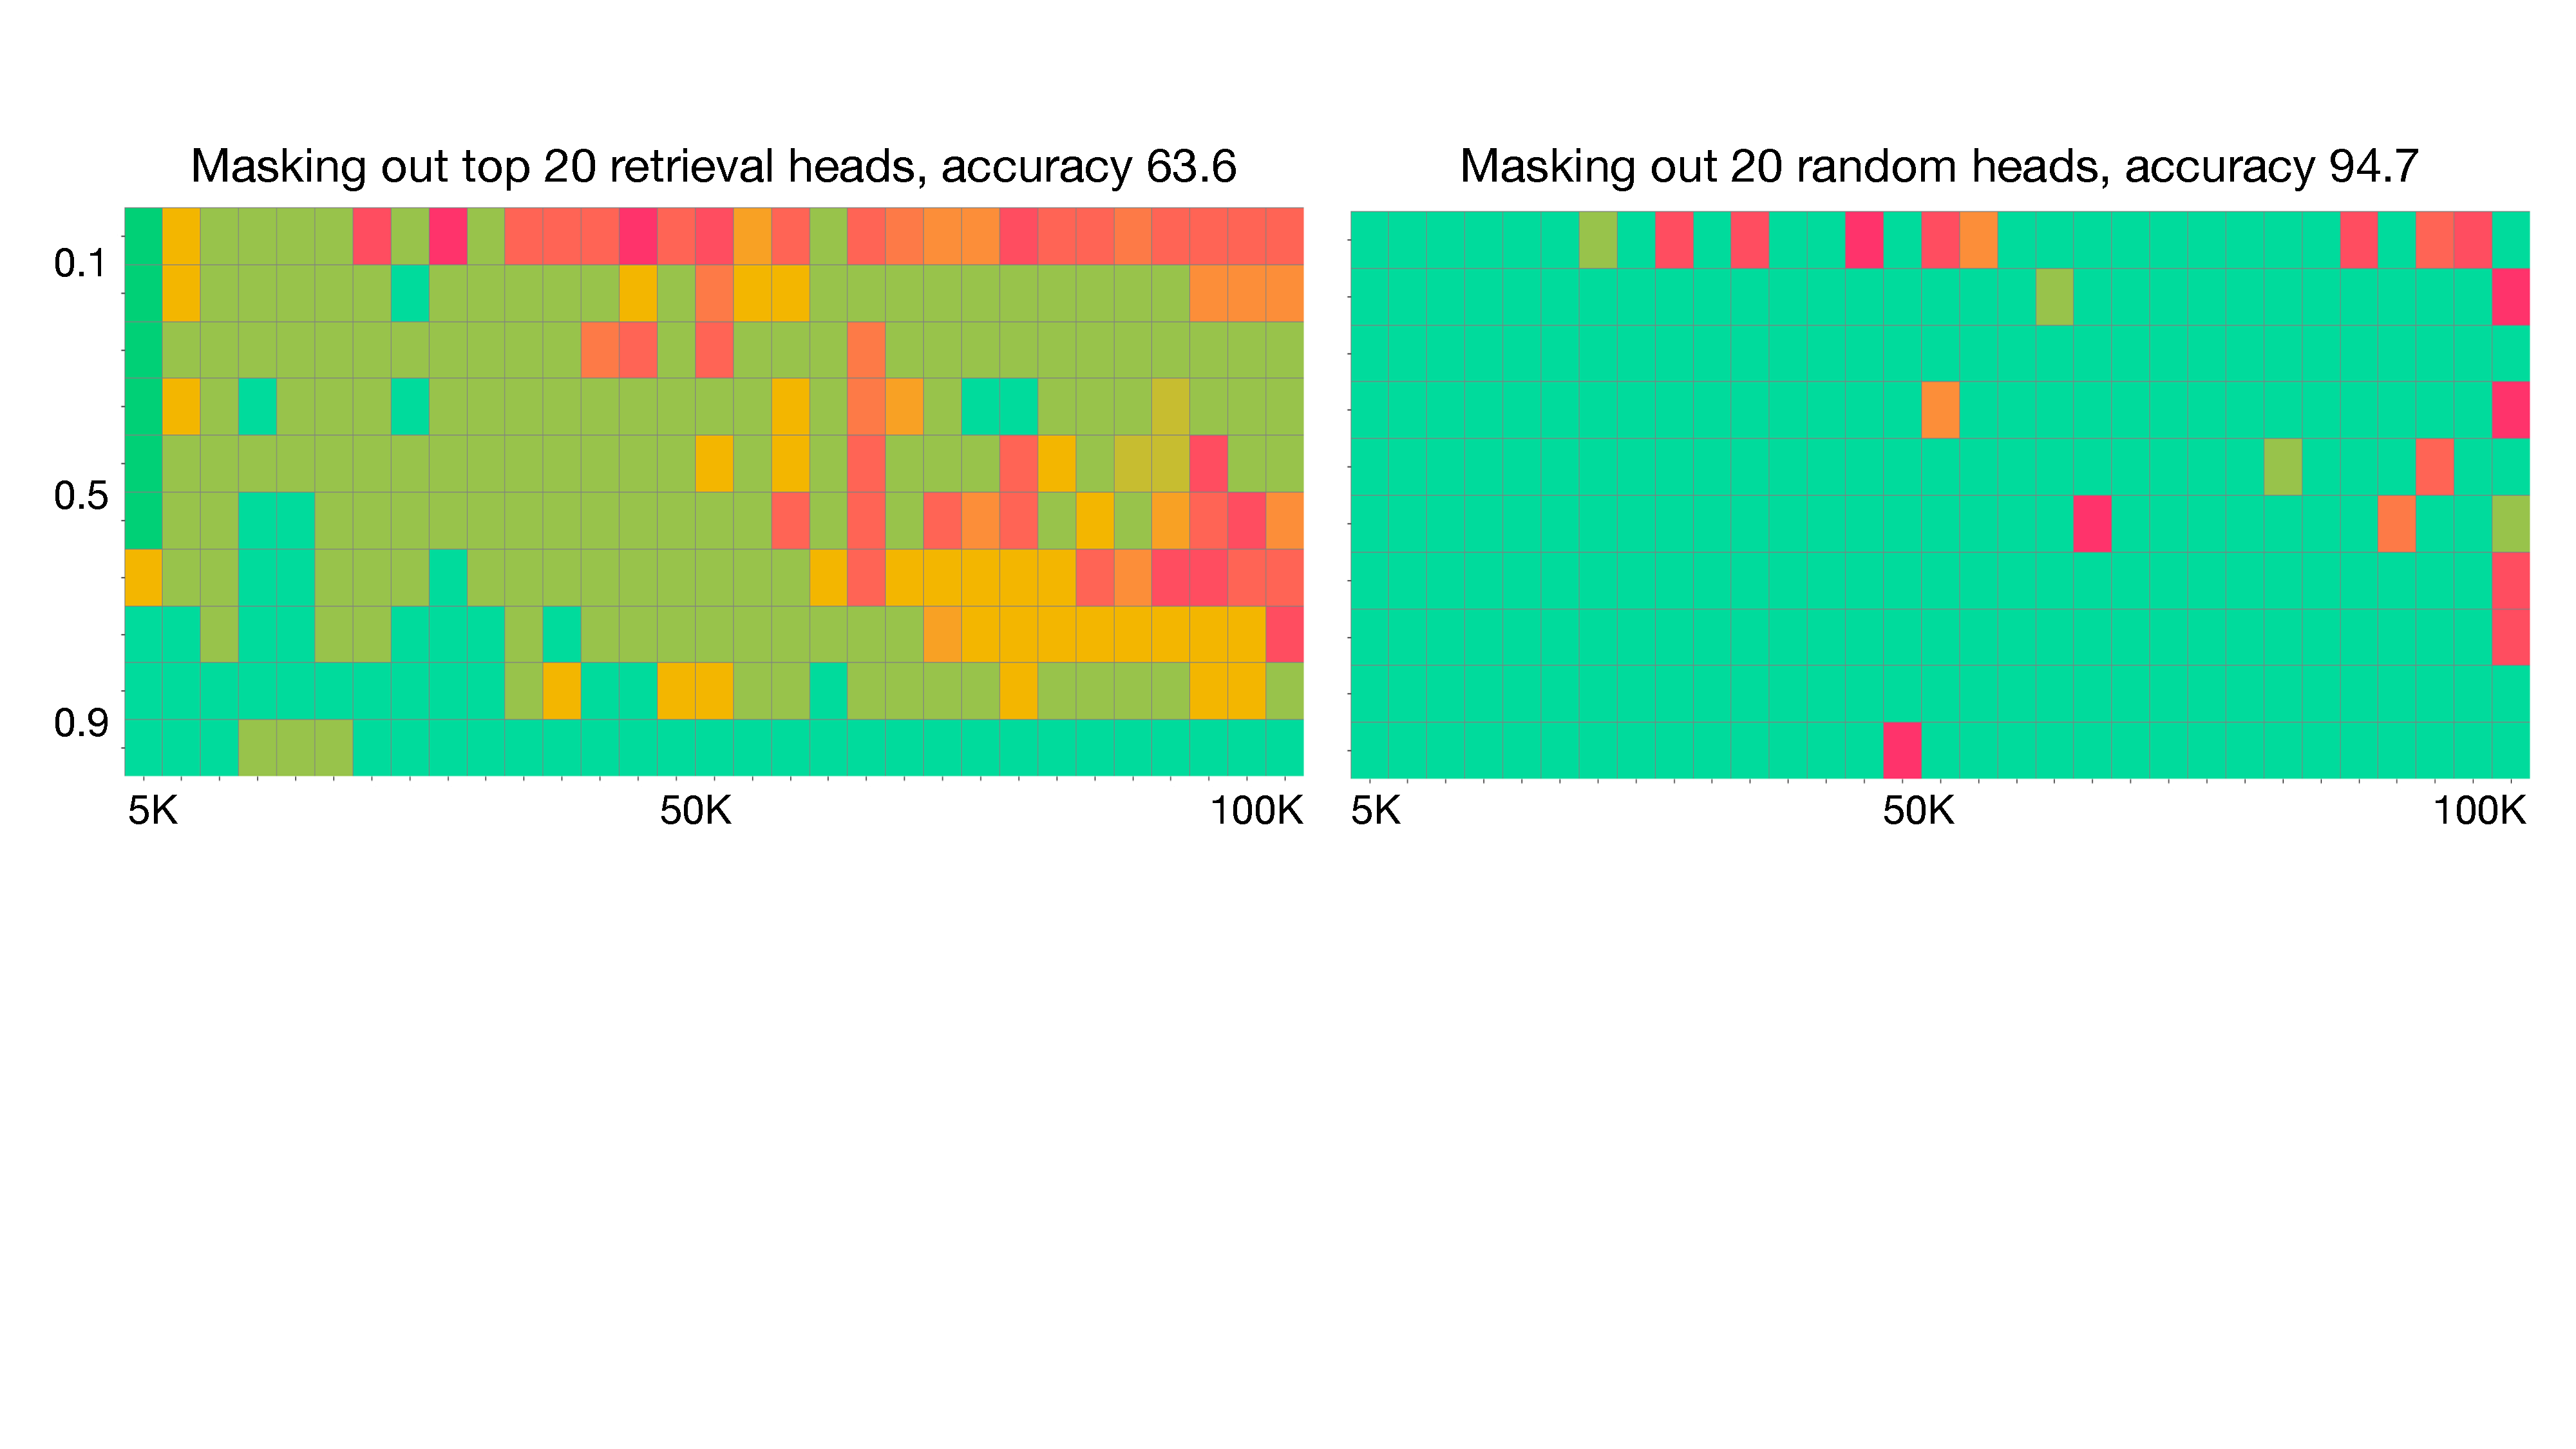
\includegraphics[width=\linewidth]{figures/retrieval_head.pdf}
  \caption{Retrieval heads are the heads that redirect information from the input to the output. Left: masking out the top retrieval heads of LLaMA 2 7B 80K, its Needle-in-a-Haystack performance drops significantly, and the model hallucinates during decoding. Right: masking out random non-retrieval heads does not influence the model's needle-in-a-haystack behavior. 
  We further note that the retrieval head only influence factuality but not the language capability: when they are masked, the model hallucinates by saying ``go to the beach'', which is still a fluent sentence, but not factual (as the correct answer is ``eating a sandwich at Dolores park.'').
  }
  \label{fig:retrieval_head}
\end{figure*}
